\documentclass[conference]{IEEEtran}
% Phase 1 report: Air Quality Forecasting via Gradient Boosting (Project 19).
% Compile from this folder with: pdflatex main && bibtex main && pdflatex main && pdflatex main
% Figures are read from ../results/figures/ (generated by the notebooks).

\usepackage{amsmath,amssymb}
\usepackage{graphicx}
\usepackage{booktabs}
\usepackage{siunitx}
\usepackage{cite}
\usepackage{url}
\graphicspath{{../results/figures/}}
\sisetup{detect-all}
\newcommand{\ugm}{\si{\micro\gram\per\cubic\metre}}

\begin{document}

\title{One-Hour-Ahead PM2.5 Forecasting in Beijing with Gradient-Boosted Trees: A Leakage-Controlled Comparison Against Naive Baselines}

\author{\IEEEauthorblockN{Animesh Kumar Rai}
\IEEEauthorblockA{Project 19 --- Phase 1 (Machine Learning)}}

\maketitle

\begin{abstract}
We forecast hourly PM2.5 concentration one hour ahead at the US Embassy in Beijing using the public UCI Beijing PM2.5 dataset (2010--2014). Every input is restricted to information available at the forecast issuance time, splits are chronological and assigned by target time, and all models are scored on an identical set of hours. Persistence is a strong baseline (test R\textsuperscript{2} = 0.944), while a 24-hour seasonal-naive forecast is worse than the mean (R\textsuperscript{2} = $-0.12$), which we explain analytically. An XGBoost model that predicts the \emph{change} from the current value, rather than the level, and is tuned only on 2013 expanding-window folds, reduces test-year MAE from 11.93 to 10.96~\ugm{} ($-8.1\%$) and RMSE from 22.03 to 19.96~\ugm{} ($-9.4\%$). It wins in all 12 test months, and the Diebold--Mariano test rejects equal accuracy ($p < 10^{-6}$). Error analysis shows that the gain comes from anticipating falls in concentration (associated with north-westerly wind onset) and from moderate levels; XGBoost does not improve on persistence for sudden rises or for concentrations above 250~\ugm{}.
\end{abstract}

\begin{IEEEkeywords}
PM2.5, air quality forecasting, XGBoost, gradient boosting, persistence baseline, time-series cross-validation, Diebold--Mariano test
\end{IEEEkeywords}

%=====================================================================
\section{Introduction}
Fine particulate matter (PM2.5) is a major health risk; the 2021 WHO guideline sets a 24-hour mean level of 15~\ugm{} \cite{who2021aqg}. Beijing frequently exceeds this by an order of magnitude, so short-term forecasts are useful for public warnings and exposure reduction.

At a one-hour horizon, PM2.5 is highly autocorrelated, and the naive forecast ``next hour equals this hour'' (persistence) is difficult to beat. Reported gains of machine learning models are therefore only meaningful relative to such baselines and under evaluation protocols that prevent information from the future leaking into the inputs or the model selection.

This work asks a deliberately narrow question: \emph{under a leakage-controlled protocol, how much does a gradient-boosted tree model improve on naive baselines for one-hour-ahead PM2.5, and where does it fail?} The contributions are:
\begin{itemize}
\item a forecasting protocol with an explicit issuance time, target-time split assignment, a common evaluation set and expanding-window backtesting;
\item a decoding of the dataset's cumulative wind variable into hourly wind speed, which became the second most important input;
\item an analytical explanation of baseline performance ($R^2 \approx 2\rho_k - 1$);
\item a formulation study showing that predicting the hourly change is essential for trees to beat persistence;
\item a single, frozen-configuration test evaluation with significance testing and error analysis by level and by direction of change.
\end{itemize}

%=====================================================================
\section{Related Work}
\textbf{Forecasting approaches.} Bai \emph{et al.} \cite{bai2018} review air pollution forecasting and group methods into statistical, artificial-intelligence and numerical (chemical transport) approaches, plus hybrids that combine them. This work belongs to the AI/statistical family and uses only station-level history and observed weather.

\textbf{The dataset.} Liang \emph{et al.} \cite{liang2015} introduced the Beijing PM2.5 data used here \cite{uci_beijing}. They proposed a statistical adjustment of PM2.5 for meteorological conditions and found that, after adjustment, concentrations in 2013 and 2014 were significantly \emph{higher} than in 2012. This is a warning that raw year-to-year comparisons conflate emissions with weather.

\textbf{Machine learning for PM2.5.} Li \emph{et al.} \cite{li2017lstm} proposed an extended LSTM (LSTME) using data from 12 Beijing stations with meteorological and timestamp inputs, and reported that it outperformed ARMA, SVR, TDNN and a standard LSTM for one-hour predictions. Zhong \emph{et al.} \cite{zhong2021lightgbm} used the gradient-boosting library LightGBM to estimate hourly PM2.5 across China from meteorological data, training on 2016--2018 and reporting R\textsuperscript{2} = 0.75 on 2019. These studies motivate tree ensembles and recurrent networks; our study adds a strict comparison against naive baselines on a single station.

\textbf{Gradient boosting.} Friedman \cite{friedman2001} framed boosting as gradient descent in function space with regression trees as base learners. XGBoost \cite{chen2016xgboost} adds a regularised objective, second-order optimisation, sparsity-aware split finding (used here for missing inputs) and an efficient histogram algorithm.

\textbf{Evaluation methodology.} Tashman \cite{tashman2000} analyses out-of-sample testing and contrasts fixed-origin with rolling-origin evaluation. Bergmeir and Ben\'itez \cite{bergmeir2012} study cross-validation for time series and recommend blocked schemes over random splits. Hyndman and Athanasopoulos \cite{hyndman2021fpp3} emphasise naive benchmarks and time-series cross-validation. To test whether two forecasts differ in accuracy we use the Diebold--Mariano test \cite{diebold1995} with a Newey--West long-run variance \cite{newey1987}.

%=====================================================================
\section{Data}
The dataset \cite{uci_beijing} contains 43,824 hourly records from 2010-01-01 00:00 to 2014-12-31 23:00: PM2.5 (\ugm{}) from the US Embassy and dew point, temperature, pressure, combined wind direction (NE, NW, SE, calm/variable), cumulated wind speed, and cumulated hours of snow and rain from Beijing Capital International Airport. The raw file is kept read-only and verified by SHA-256 on every load.

\textbf{Quality.} The hourly index is complete, unique and ordered. Only PM2.5 is missing: 2,067 hours (4.7\%) in 214 gaps, from single hours to 155 hours; missingness is 6--8\% in 2010--2012 and about 1\% in 2013--2014. Values up to 994~\ugm{} coincide with known episodes (e.g.\ Chinese New Year) and are kept.

\textbf{Cumulative variables.} The wind variable accumulates speed while the direction is unchanged and resets when it changes; we verified this exactly and decode the hourly speed as the within-run increment.

\textbf{Exploratory findings.} PM2.5 is right-skewed (median 72, 99th percentile 420~\ugm{}). The autocorrelation is 0.96 at lag 1 but only 0.39 at lag 24 and about 0.02 at lag 168, and the partial autocorrelation is negligible beyond lag 2 (Fig.~\ref{fig:acf}). The daily cycle differs by season (overnight peaks in winter and autumn, morning peaks in spring and summer). North-westerly wind is associated with clean air (median 31~\ugm{}) and calm/variable wind with high concentrations (median 98~\ugm{}).

\begin{figure}[t]
\centering
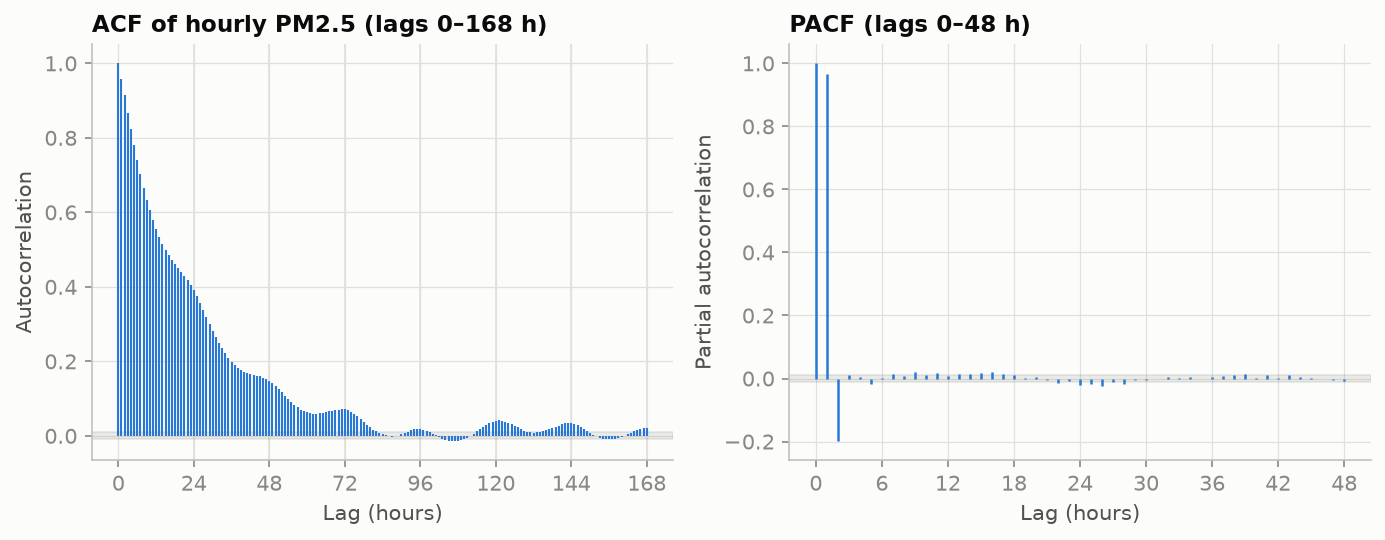
\includegraphics[width=\columnwidth]{eda_06_acf_pacf.png}
\caption{ACF (left) and PACF (right) of hourly PM2.5, 2010--2014.}
\label{fig:acf}
\end{figure}

%=====================================================================
\section{Methodology}
\subsection{Forecasting protocol}
The forecast is issued at the end of hour $t$, and the target is $y_t = x_{t+1}$, the PM2.5 concentration one hour later. Inputs may use observations at hours $\le t$ and calendar attributes of $t+1$; realised future weather is excluded. Each sample is assigned to the split containing its \emph{target} hour: training 2010--2012, validation 2013, test 2014 (Fig.~\ref{fig:protocol}). Whole calendar years keep every season in each split.

All models are scored on a \emph{common evaluation set}: hours where the target, $x_t$ and $x_{t-23}$ are observed, so both baselines are defined (train 23,452; validation 8,563; test 8,531 hours). Targets are never imputed. Input gaps are left missing rather than interpolated, because interpolation uses values after $t$.

\begin{figure}[t]
\centering
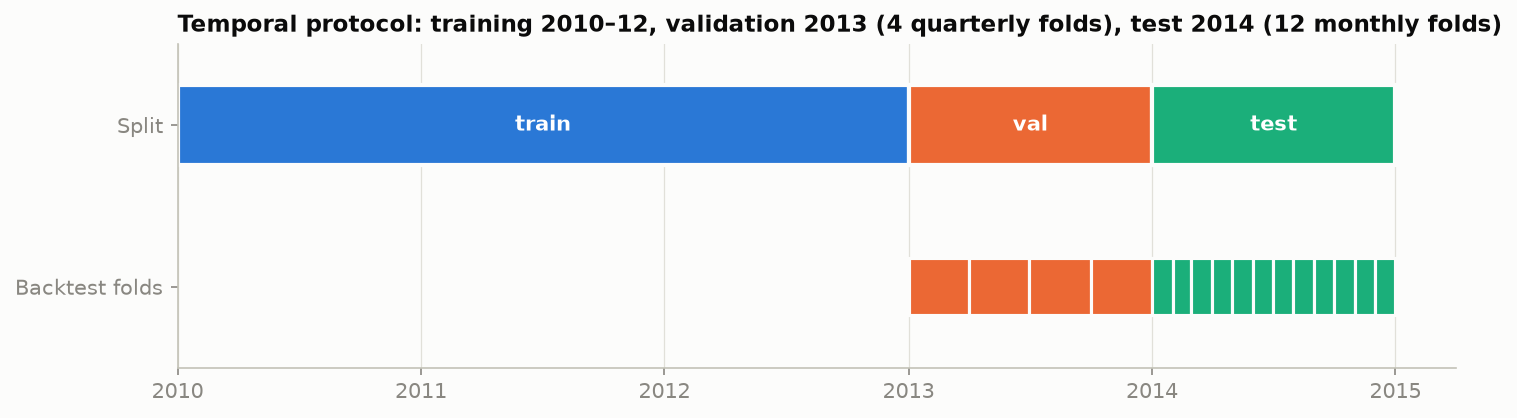
\includegraphics[width=\columnwidth]{protocol_01_timeline.png}
\caption{Temporal protocol: tuning folds (2013 quarters) and final evaluation folds (2014 months).}
\label{fig:protocol}
\end{figure}

\subsection{Features}
Thirty-seven features are computed from data at hours $\le t$:
\begin{itemize}
\item PM2.5 lags $x_{t-k}$ for $k \in \{0,1,2,3,6,12,23\}$, chosen from the ACF/PACF;
\item the last hourly change;
\item trailing means and standard deviations over 3, 6, 12 and 24 hours;
\item hours since the last PM2.5 observation;
\item observed weather: dew point, temperature, pressure, temperature--dew-point spread, and 3-hour tendencies;
\item wind: decoded hourly speed, persistence of the current direction, and a one-hot direction;
\item precipitation counters;
\item cyclical hour and month and the day of week of $t+1$.
\end{itemize}
A perturbation test confirmed causality: randomising all rows after $t$, at 30 random cut points, left every feature at times $\le t$ unchanged.

\subsection{Baselines}
Persistence predicts $\hat{y}_t = x_t$. Seasonal-naive predicts $\hat{y}_t = x_{t+1-24}$. For a stationary series with variance $\sigma^2$ and lag-$k$ autocorrelation $\rho_k$, the naive lag-$k$ forecast has
\begin{equation}
\mathbb{E}\left[(x_{t+k}-x_t)^2\right] = 2\sigma^2(1-\rho_k) \;\Rightarrow\; R^2 \approx 2\rho_k - 1,
\label{eq:naive}
\end{equation}
so a naive forecast is worse than the mean whenever $\rho_k < 0.5$.

\subsection{XGBoost}
XGBoost minimises $\sum_i \ell(y_i,\hat{y}_i) + \sum_k \Omega(f_k)$ with $\Omega(f) = \gamma T + \tfrac{1}{2}\lambda\lVert w\rVert^2$, where $T$ is the number of leaves and $w$ the leaf weights \cite{chen2016xgboost}; we use squared loss. Because each tree is piecewise constant, approximating the near-identity map $x_t \mapsto x_{t+1}$ requires many splits. We therefore compare three target formulations: level, $\log(1+x_{t+1})$, and the \emph{change} $x_{t+1} - x_t$, with $x_t$ added back at prediction time.

\subsection{Tuning and evaluation}
Hyperparameters were selected by lowest mean RMSE over four expanding-window folds (the quarters of 2013), using 40 random configurations. The 2014 test year was not used until the configuration was frozen. The final evaluation refits the model before each 2014 month on all earlier targets (12 folds), and a single fit on 2010--2013 is reported as a secondary result. Metrics are MAE, RMSE and R\textsuperscript{2} on the original scale. Equal accuracy is tested with the Diebold--Mariano statistic \cite{diebold1995}, $\mathrm{DM} = \bar{d}/\sqrt{\hat{V}/n}$ with $d_t = L(e_{1,t}) - L(e_{2,t})$ and a Newey--West variance $\hat{V}$ with 24 lags \cite{newey1987}.

%=====================================================================
\section{Results}
\subsection{Validation (2013)}
With identical hyperparameters, the level and log formulations did not beat persistence on mean fold RMSE (23.79 and 24.31 vs.\ 23.70~\ugm{}), whereas the change formulation reached 21.80. Tuning lowered this to 21.41; the five-seed standard deviation was about 0.04, so the gain exceeds run-to-run noise but is small. Pooled over 2013, XGBoost achieved MAE 12.26 and RMSE 22.53~\ugm{} against 13.18 and 24.87 for persistence.

\subsection{Test (2014)}
Table~\ref{tab:test} gives the single test evaluation. XGBoost improves on persistence by 8.1\% (MAE) and 9.4\% (RMSE), the same relative RMSE gain as on validation, and is better in all 12 months on both metrics (Fig.~\ref{fig:monthly}). The Diebold--Mariano test rejects equal accuracy against persistence for squared loss ($\mathrm{DM} = -5.10$, $p = 3.4\times10^{-7}$) and absolute loss ($\mathrm{DM} = -8.64$, $p = 5.8\times10^{-18}$). Refitting monthly gave no benefit over a single fit (RMSE 19.96 vs.\ 19.97). Seasonal-naive has R\textsuperscript{2} below zero, consistent with (\ref{eq:naive}): on training data, $\rho_{24} = 0.384$ predicts $-0.231$ and $-0.222$ was observed.

\begin{table}[t]
\centering
\caption{Test-year results (2014, 8,531 common hours)}
\label{tab:test}
\begin{tabular}{lccc}
\toprule
Model & MAE (\ugm{}) & RMSE (\ugm{}) & R\textsuperscript{2} \\
\midrule
Persistence & 11.93 & 22.03 & 0.944 \\
Seasonal-naive (24 h) & 67.30 & 98.75 & $-0.121$ \\
XGBoost (change target) & \textbf{10.96} & \textbf{19.96} & \textbf{0.954} \\
\bottomrule
\end{tabular}
\end{table}

\begin{figure}[t]
\centering
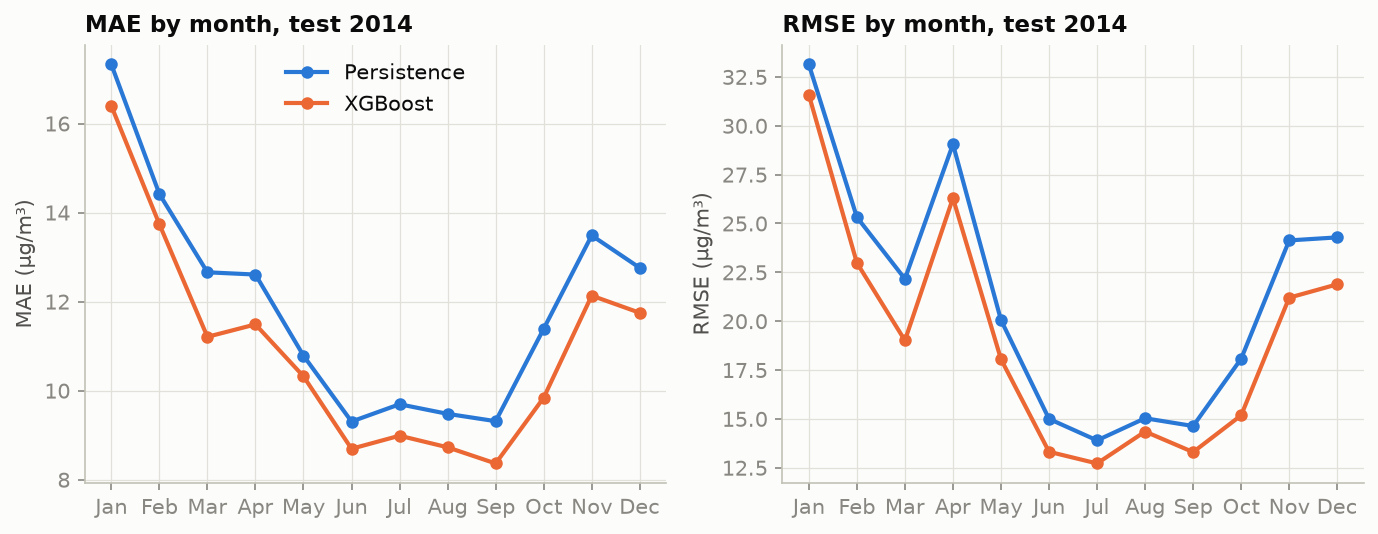
\includegraphics[width=\columnwidth]{test_01_monthly.png}
\caption{Monthly MAE and RMSE on the 2014 test year (expanding-window refits).}
\label{fig:monthly}
\end{figure}

\subsection{Error analysis}
\textbf{By level} (Fig.~\ref{fig:level}). XGBoost reduces RMSE in every band up to 250~\ugm{}, but above 250~\ugm{} (7.6\% of test hours) it is slightly worse than persistence (42.0 vs.\ 41.6). It under-predicts these hours by 12.8~\ugm{} on average, and they account for 34\% of its squared error. This is the regression-to-the-mean behaviour expected from squared-loss leaf averaging.

\textbf{By direction of change.} For large falls ($\Delta \le -50$~\ugm{}, 178 hours) MAE drops from 84.7 to 60.6. For large rises ($\Delta > 50$, 91 hours) there is no gain (84.9 vs.\ 85.1). On stable hours XGBoost is slightly worse (5.0 vs.\ 4.0), the cost of predicting small changes that do not occur. A recent onset of north-westerly wind precedes 24.2\% of large-fall hours versus 13.1\% of other hours, consistent with clean-air arrivals being visible in the inputs, whereas build-ups are not.

\textbf{Residuals and importance.} The lag-1 autocorrelation of errors falls from 0.143 (persistence) to 0.003 (XGBoost). Permutation importance on 2013 ranks the current PM2.5 and the decoded hourly wind speed highest (each raising RMSE by about 2.3~\ugm{} when shuffled), followed by the 3-hour dew-point change.

\begin{figure}[t]
\centering
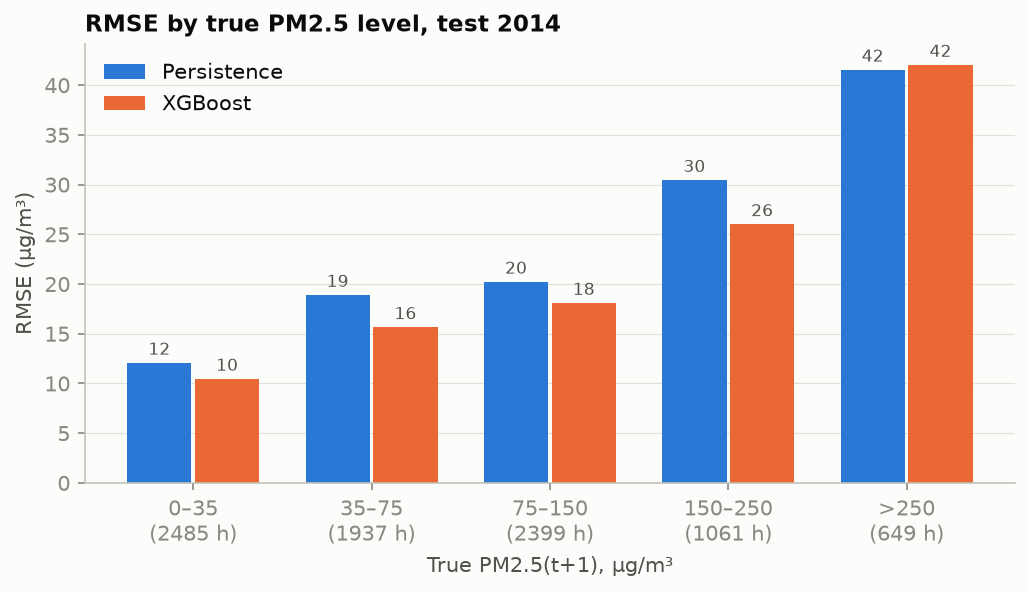
\includegraphics[width=\columnwidth]{test_02_by_level.png}
\caption{Test-year RMSE by true PM2.5 level.}
\label{fig:level}
\end{figure}

%=====================================================================
\section{Discussion and Limitations}
The improvement over persistence is real but modest, which is typical when the one-hour autocorrelation is 0.96. Framing the problem (predicting the change) mattered more than hyperparameter tuning. The model's skill is asymmetric: inputs at time $t$ reveal arriving clean air through the wind, but not the onset of pollution build-up.

\textbf{Limitations.}
\begin{itemize}
\item Results come from one station and one test year; 2014 appears easier than 2013 for both models.
\item Inputs use only observed weather; operational weather forecasts were not tested.
\item The Diebold--Mariano implementation slightly over-rejected (about 8\% at a nominal 5\%) in a simulation with autocorrelated errors, so its $p$-values are approximate, although the observed values are far below any threshold.
\item The exploratory analysis used the full period, but only for qualitative design choices.
\item Losses targeting extremes, such as quantile or tail-weighted losses, were not explored.
\end{itemize}

%=====================================================================
\section{Conclusion and Future Work}
Under a leakage-controlled protocol, XGBoost with a change target reduces one-hour-ahead PM2.5 test error by about 9\% (RMSE) relative to persistence, consistently across months and with statistical significance. However, it does not improve forecasts of extreme concentrations or sudden rises. Phase~2 will evaluate an LSTM \cite{hochreiter1997} under the identical protocol, focusing on whether sequence models anticipate build-ups and extremes better, and will consider losses that weight high concentrations.

All code, the exact environment and the results are reproducible: re-running every notebook in a freshly built environment regenerated all metric and prediction files byte for byte.

\bibliographystyle{IEEEtran}
\bibliography{references}

\end{document}
